\documentclass{standalone}
\usepackage{tikz}
\usetikzlibrary{calc}

\begin{document}

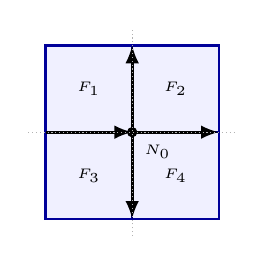
\begin{tikzpicture}[scale=1.1, every node/.style={font=\small}]
% Draw four squares
\draw[thick,fill=blue!6,draw=blue!60!black] (-1,0) rectangle (0,1);
\draw[thick,fill=blue!6,draw=blue!60!black] (0,0) rectangle (1,1);
\draw[thick,fill=blue!6,draw=blue!60!black] (-1,-1) rectangle (0,0);
\draw[thick,fill=blue!6,draw=blue!60!black] (0,-1) rectangle (1,0);

% Central vertex
\fill (0,0) circle (1.7pt) node[below right,xshift=1pt,yshift=-1pt] {\tiny $N_0$};

% \draw[very thick,->,>=latex] (-1,0) -- (0,0)
%   node[midway, below+ 0, yshift=-2pt] {\tiny $E_a$};
% \draw[very thick,->,>=latex] (0,0) -- (1,0)
%   node[midway,below+ 0.6, yshift=-2pt] {\tiny $E_b$};
% \draw[very thick,->,>=latex] (0,0) -- (0,1)
%   node[midway,right + 0.5, xshift=2pt] {\tiny $E_c$};
% \draw[very thick,->,>=latex] (0,0) -- (0,-1)
%   node[midway,right+ 0.7, xshift=2pt] {\tiny $E_d$};

\draw[very thick,->,>=latex] (-1,0) -- (0,0);
\draw[very thick,->,>=latex] (0,0) -- (1,0);
\draw[very thick,->,>=latex] (0,0) -- (0,1);
\draw[very thick,->,>=latex] (0,0) -- (0,-1);

\node at (-0.5,0.5) {\tiny $F_1$};
\node at (0.5,0.5)  {\tiny $F_2$};
\node at (-0.5,-0.5) {\tiny $F_3$};
\node at (0.5,-0.5)  {\tiny $F_4$};
\draw[densely dotted,gray!60,line width=0.4pt] (-1.2,0)--(1.2,0);
\draw[densely dotted,gray!60,line width=0.4pt] (0,-1.2)--(0,1.2);
\end{tikzpicture}

\end{document}
